\documentclass[tikz, margin=0.25mm]{standalone}

\begin{document}
    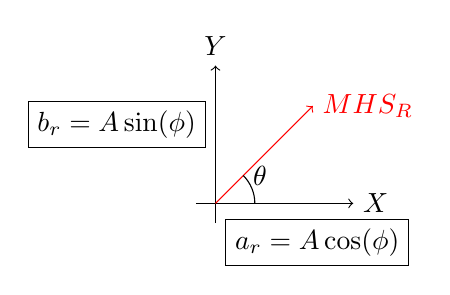
\begin{tikzpicture}
    %axis
        \draw[->]   (-.25,0) -- + (2,0) node[right] {$X$} ;
        \draw[->] (0,-.25) -- +(0,2) node[above] {$Y$};
    %result
    \draw[->, red] (0,0) -- (45:1.75) node[right]{$MHS_R$};
    \draw[] (.5,0) arc (0:45:.5) node[right]{$\theta$};
    \node[draw,below,right](ar) at (0.125,-0.5) {$a_r=A\cos(\phi)$};
    \node[draw,above,left](br) at (-0.125,1) {$b_r=A\sin(\phi)$};
    \end{tikzpicture}  
\end{document}